% ---------------------------------------------------
% ----- Chapters of the template
% ----- for Bachelor-, Master thesis and class papers
% ---------------------------------------------------
%  Created by C. Müller-Birn on 2012-08-17, CC-BY-SA 3.0.
%  Freie Universität Berlin, Institute of Computer Science, Human Centered Computing. 
%
% TODO remove 2 - to use auto numbering
\chapter{User research and analysis}
\label{chap:research}


% Due to the limited size of the user group, the goal was not to gain <TODO> with high diversity of their demographics, but to have information saturation from fewer but more valuable insights into peolpe with diffrent workflows.

Cites:
\begin{itemize}
  \item \cite{Ross:2016} why companies dont conduct user research
\end{itemize}

Over ten years after the publication of Tomer Sharon's book ''It's our Research'', the listing of qoutes in the introduction about user research in software companies still feel as relevant as ever.
\\
''Yeah, but this study will delay our launch date.'', ''Yeah, but we can't learn much from only five participants.'', ''Yeah, but research sounds so academic.'' \cite[p. 4]{Sharon:2012mk} are only some of the statements that according to Sharon are often heard in software companies when discussing if UX research should be conducted.
\\
The common pressure from different stakeholders often leads to quick implementation of features and workflows without first investing time to figure the user's needs out, which may be faster in the beginning, but can badly impact the user's acceptance of the product due to cumbersome and slow workflows,
in the worst case leading to the user not using the product anymore.

To counteract this, it is crucial to conduct and evaluate user research methods, which is what I did for the development of the UI builder.

A starting point for qualitative user research is to define the goals through the help of the SMART criteria, which provide guidelines and formulated goals during research.

For the project, I defined the SMART criteria as following:

\begin{itemize}
  \item \textbf{specfic} - improve the workflow of users modifying dynamic resources for the Purple Experience.
  \item \textbf{measurable} - interviews after testing period concerning working speed, confidence and joy when editing resources, automated user tracking
  \item \textbf{assignable} - research and implementation will mostly be conducted by me, with input from CTO \& product owner, connections to external users through customer service team
  \item \textbf{realistic} - new software platform which reacts quicker, prvides more safety regarding errors and is scalable and extensible in the future. Limiting factors are time (as I only have three months for the first phase, including writinh this thesis)
  \item \textbf{time-related} - the new software should have at least the same feature set and be usable by company-internal users until the end of 2022
\end{itemize}

\section{Identifying and categorizing users and user groups}
\label{sec:user-groups}
In order to effectively design and implement the UI editor, it is crucial to understand the needs and preferences of the various users and user groups who will be using the tool.
Therefore, the first step in the user research process was to identify and categorize the different users and user groups who will be using the editor.

In a later chapter (\ref{sec:personas}), I'll build concrete Personas for the different user groups utilizing the information gained from the interviews.
\\
Because we already have existing users that work with the previous editors and other tools from the ecosystem, it was relatively easy to collect a list of internal and extneral users, which either I personally knew or I could write a short message asking about if and how they use existing tools and modify dynamic resources.
I see that this won't be as easy when dealing with a larger user base or primary external customers, when this first step probably requires more effort to collect a user overview upfront.
\\
With a list of many of the users, I started grouping them to understand the characteristics and needs of each user group, through which can ensure that the UI editor is tailored to their specific requirements and can be used effectively by all users\footnote{When I refer to ''all users'', I mean the group of users that are expected to work with the tool. There is an expected technical and domain specific base knowledge that the Editor won't cover}.
\\
I derived the follwoing commomn factors from the users, which made the communication and categorization a lot easier.

\begin{itemize}
  \item \textbf{quantitative usage} There were users who relied on the tools for most of their work, while others like the external customers accessed the tool a few times a year.
  \item \textbf{common tasks} I roughly categorized the common tasks into three groups:
    \subitem \textbf{Heavy configuration} Mostly internal devs used the tools to build new apps and websites from scratch (or derived from exisiting apps), making many modifications, from structural changes to the seperate views, menus, data sources and more, over styling and translating messages to diffrent languages.
    \subitem \textbf{Moderate configuration} Project devs and customer support people copy resources from existing apps and adapt them for new brands, which often includes changing colors and logos, adapting texts or switching authentification flows.
    \subitem \textbf{Small changes} External customers often only use the tools to exchange some ads, translations or logos, which affects a small set of files.
  \item \textbf{expertise} 
  %<kann man bei schlechter software gut erkennen, leute mit viel erfahrung checken sachen, aber ist für neue nicht intutitiv>
    \subitem \textbf{Technical} Depending on the area of education and working time in the web development industry, the expertise about web technologies, languages like CSS and JSON and often also intuition differs between users.
    \subitem \textbf{Domain- and Platform Specific} There is a lot of vocabulary, functionality of the Purple Experience and other systems as well as permutations of configurations that users learn with time.
\end{itemize}

% ... more
\section{Qualitative user resarch}

The existing user base enabled me easy access to subjects for qualitative user research methods.
Using one or multiple ways of Triangulation \cite[p. 264]{Interactiondesign:2019ys} can strengthen the significance of the research outcome. Limitations of a method or source can be removed by variation of those, resulting in a less distorted picture.
Therefore I used metholodical triangulation (using multiple data gathering techniques) as well as triangulation of data (collecting data from different people and different sources).
Moderated observations combined with interviews proofed to be a good fit for this case study, as they are interaction driven and the observer can react directly on behaviours / emerging topics and steer the process.
This stands is contrast to more passive methods I found like passive observations or user recording and tracking analysis, where the outcome only depends on the
prepared question / task and the users behaviour and which can't adapt to changed circuumstances etc. during the application.
\\\\
The chosen structure for the observations and interviews looks as following:

\begin{description}
  \item [Introduction (\texttildelow 5min)] used to explain the circuumstances and the goal of the session, how we proceed, which data I will collect and how I will evaluate the data afterwards.
  \item [Moderated Observation (10-15min)] have the observed perform specific tasks in a prepared environment
  \item [Semistructured Interview (\texttildelow 15min)] ask prepared questions as well as open ones and discuss observation situation
\end{description}
The reason for Interview following the Observation is, that the observer and observed can discuss the situations or issues occured during the Moderated Observation before,
which was a good point of entry into the open dialog after the mandatory prepared questions were asked. The other way around, I'd have no way to react to workflow and potential problems the observed encountered during the tasks.
\\
As I had no prior experience conducting these methods with an scientific approach, it was important to me to test the whole process before scheduling all the other meetings. One of our working students agreed to be a test candidate and we went through the tasks and questions I planned, after which he gave me feedback.
Testing the methods and specific questions before conducting them on a broader audience helped finding questiones that were ambiguous or lead to a lot of repetition of already known facts. For the moderated observation tasks it gave me feedback on the difficulty and time they would take for others on average, which tasks needed clearer formulations and which were already good.
\\
In total, I performed the user research on six persons, from which one was an core Purple Experience developer, two were working students from our project department, one was an developer from an different department who had worked with the software some time prior, one Customer Support Manager from our company and one external user from an publisher.

\subsection{Moderated observation}
I prepared a list of six tasks, with the last two beeing optional depending on the time left and the confidence of the user with the platform I perceived during the beginning.
That way I could present the same first tasks to every interviewee regardless of their level of knowledge, and present the last two tasks if we had enough time left.
Also, it was important that the tasks did not build on each other to prevent the observed person getting stuck because of an earlier mistake.
To me, it was more important to see a variety of tasks getting performed than one task beeing executed without errors. 
\\
In practice, I prepared an example app on our staging system, noted the link down and downloaded the initial state so that I could easily reset the enviornment after each observation.
The six tasks were
\begin{itemize}
  \item Change english app menu entry "Newsstand" to "Home" on all platforms (Web, Android and iOS)
  \item Change the Advertisement banner target on top of the home page to https://google.com 
  \item Change the exnglish text "Latest Issues" on the home page to "Read new Issues"
  \item Change color of "Read new Issues" and "Latest Articles" headers on the home page to the app's primary color.
  \item \textit{(Optional)} Add an dropdown on the home between "Read new Issues" and "Latest Articles"
    \subitem It should show all publications connected to the app
    \subitem It should set an URL parameter ''publication'' to the id when selected
    \subitem Define the reset message as ''All publications''
  \item \textit{(Optional)} Configure the filter of the ''Latest Articles'' list to only show articles from that publication
\end{itemize}

These were constructed in a way that I anticipated some errors so I could see how users tried to figure out what went wrong and fix them.
These cases then also occurred, for example the first task was often only done for one of the three platforms, the ''Latest Issues'' text was not found in the translation files or
the wrong CSS selector was used to recolor the header elements on the home page, leading to more elements beeing recolored.

The optional tasks were presented to four people, of which three solved them at least one of them successfully, only the core developer solved all six tasks completely.
With the consent of the interviewees I recorded their screens during the observation to rewatch specific actions or flows if required.
\\
TODO: noticed workflow patterns that can be improved? like file opening, switching files (quick links \& file tabs)

\subsection{Interview}

For the interview, I chose a semistructured interview as the appropriate tool. The interviewer has a list of open and closed questions, through which he can ensure that important topics are covered,
while still leaving room for deeper covering of specific points the interview might not anticipate before the interview.

\section{Quantitaive user research}

- Not used survey / questionaire -> lay down reasons why not necessary in that situation

- Tracking of user behaviours

- on site using G analytics \& squaky.ai (TODO: remove g analytics? ask Peter)
- using server logs to understand usage patterns

\section{Process and vizualize the outcomes of the initial user research phase}

\subsection{2x2 Opportunity Matrix}

This two-dimensional vizualization of a set of proposed features prooved helpful when prioritizing tasks with other stakeholders,
as it shows the (approximated) cost of implementation as well as the value the feature can have for users.

The matrix I used is a slightly modified adaption from \cite[p. 181]{LearnHCI:2020ys}, replaced the term ''idea originality'' on the x-axis with ''Value''.

\begin{figure}[ht]
	\centering
  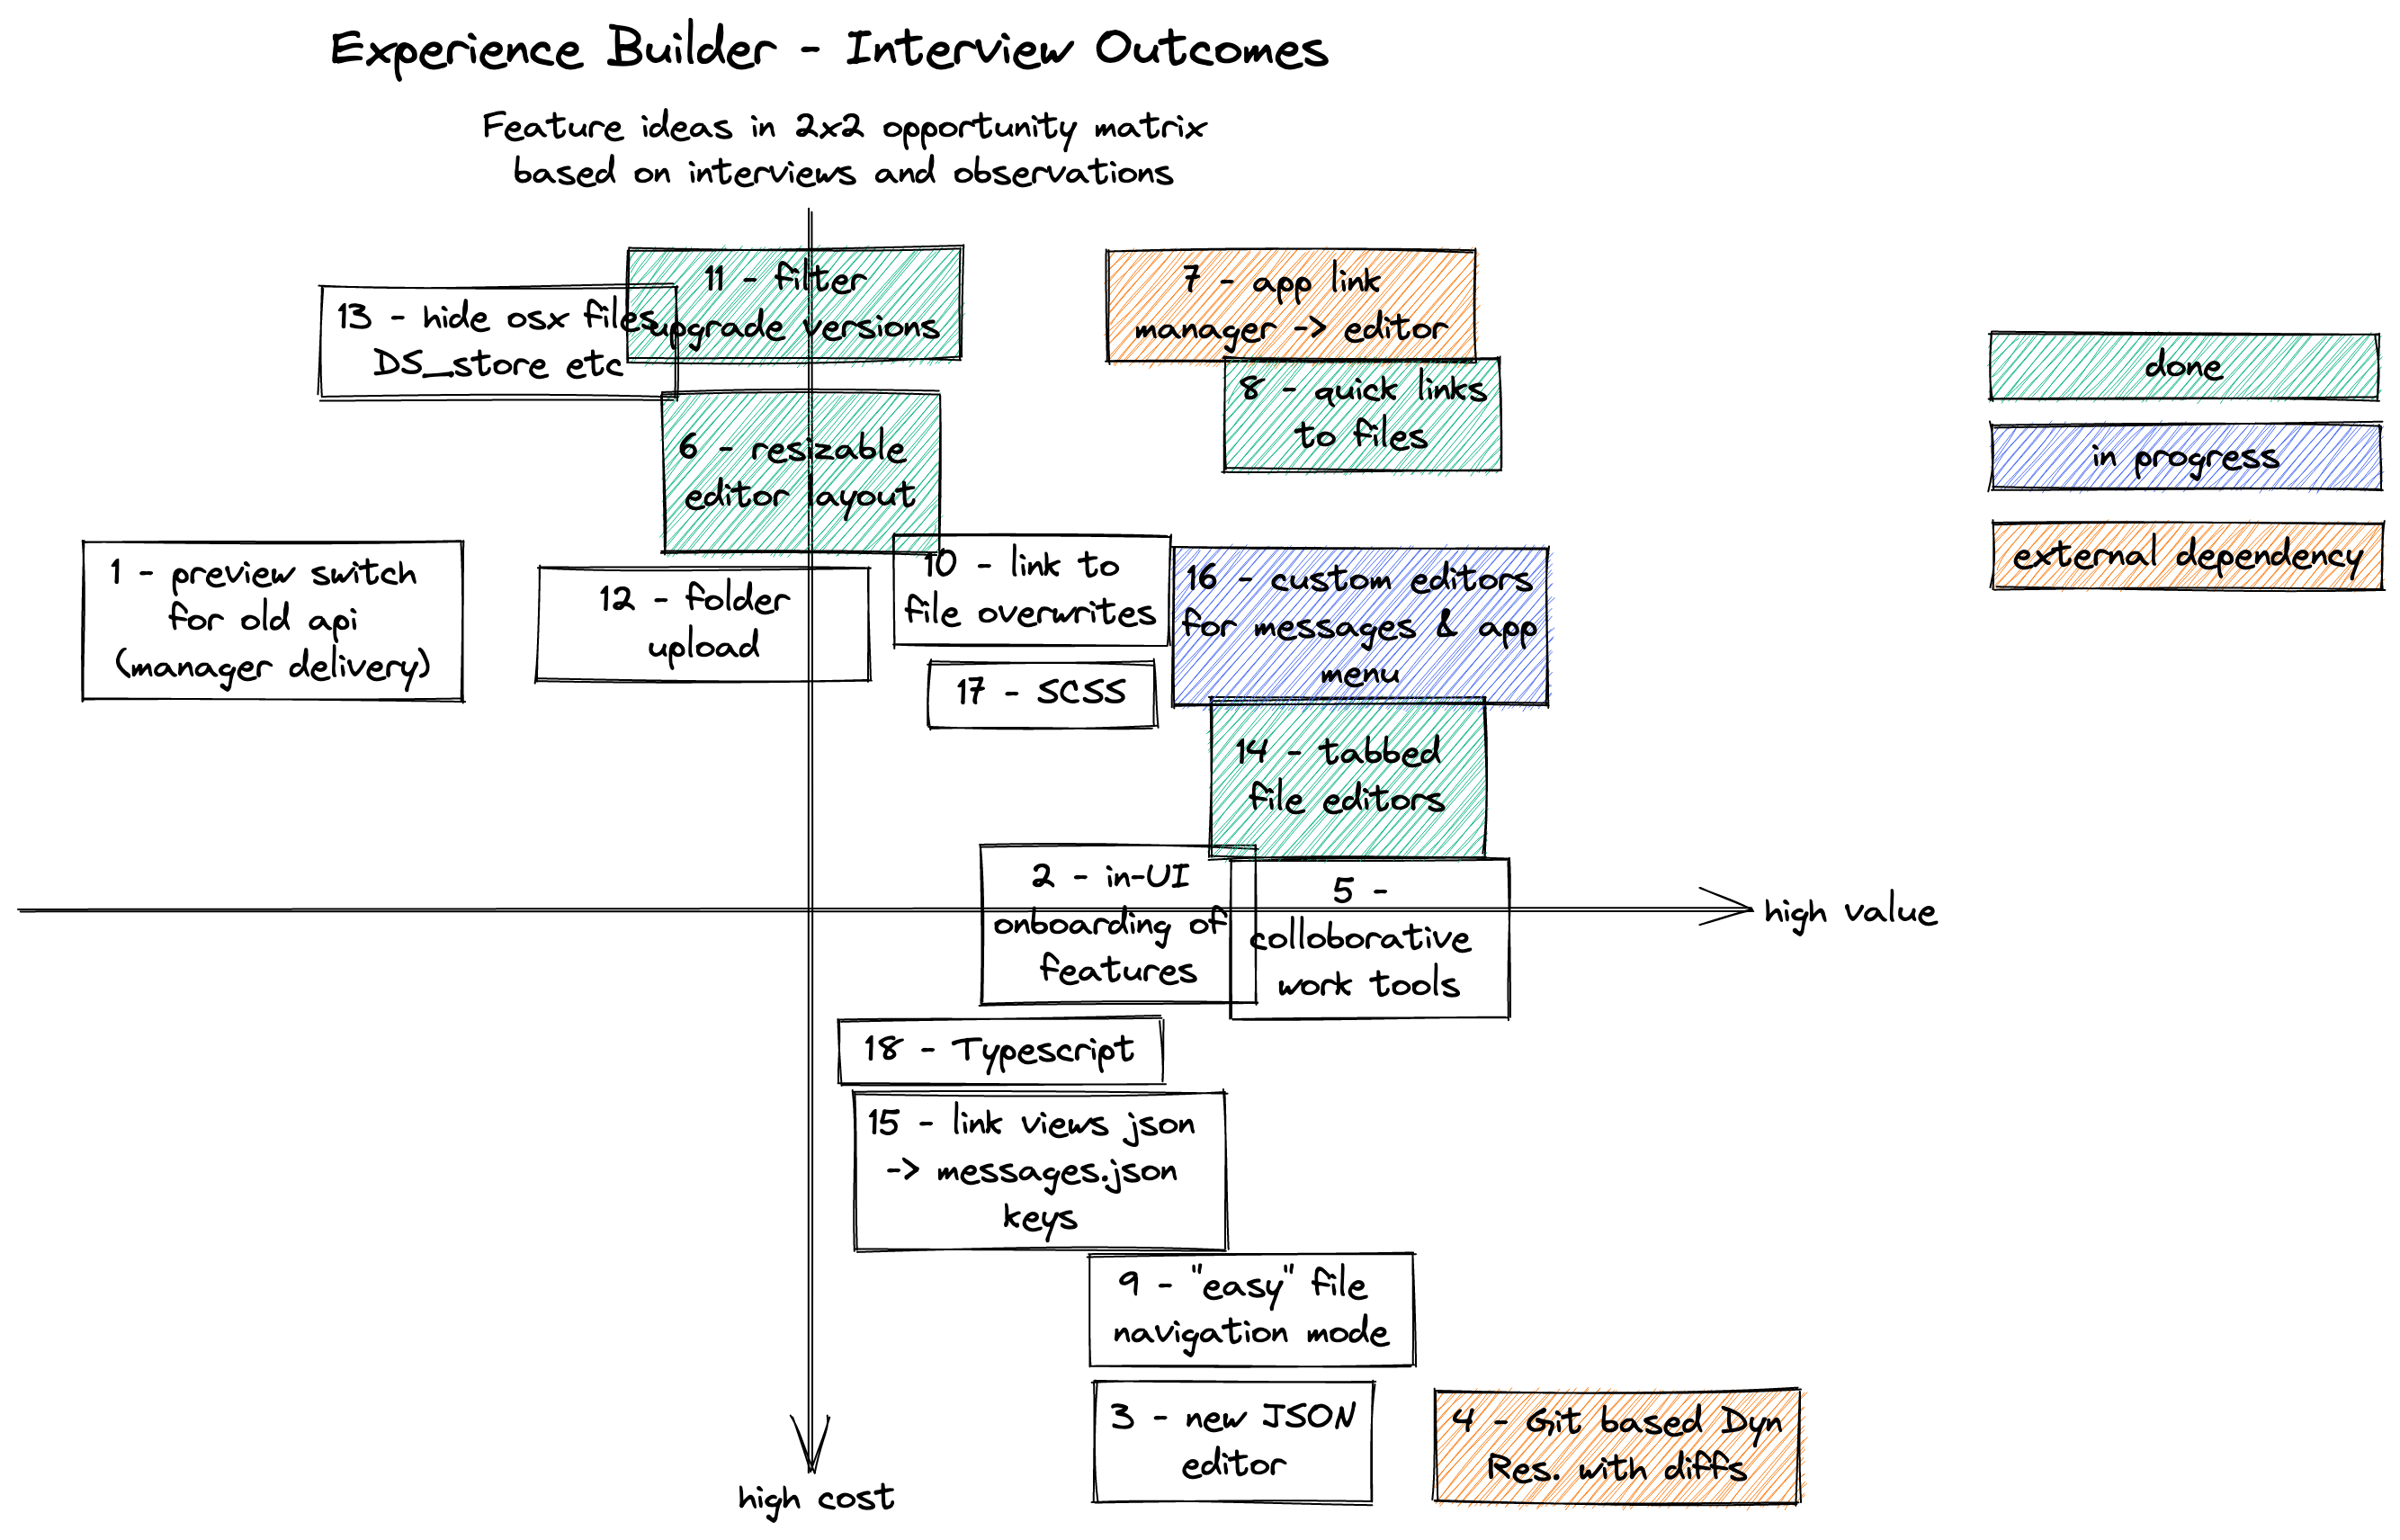
\includegraphics[width=\textwidth]{pics/feature_cost_matrix.excalidraw.png}
	\caption{2x2 Opportunity Matrix during the early phases of development}
	\label{fig:opportunitymatrix}
\end{figure}


\section{Building Personas}
\label{sec:personas}

Personas are descriptions of fictional users of the product, incorporating assumptions and optinally data for a user group.
They aim to give developers and designers more context and depict real potential users, which makes it easier for a developer to empathize with the user.
The following three Role-based Personas are derived from \ref{sec:user-groups} and the outcomes of the interviews, based on the description of Personas in \cite[pp. 403-405]{Interactiondesign:2019ys}
\\
\hrule
% Persona 1
\subsection{John - Purple Expeirence Product Developer}
\subsubsection{Background and Skills}
John (34) is a senior Angular Web Developer at Sprylab, working there for two years. He was born in Berlin and lives in Lichterfelde with his wife and mostly works from home. He is passionate about Angular, Typescript and Developer Experience in general, studied Computer Science at the Beuth Hochschule and hosts Angular conferences.
\\
\subsubsection{Goals and work with the Editor}
\begin{itemize}
  \item Test newly developed features and the related configurations
  \item Configure test apps for development and QA purposes
  \item Support in case Project Developers like <TODO> encounter problems
  \item John works with the editor multiple times a week
\end{itemize}

\hrule
% Persona 2
\subsection{Steffi - Project Developer}
\subsubsection{Background and Skills}
Steffi (23) studies media informatics and works as a working student at Sprylab since a year. This is her first job in the industry and she is learning new things every day. Her skills include writing CSS and understanding modern web technologies, but she still struggles using native and custom debugging tools if something goes wrong.  
\\
\subsubsection{Goals and work with the Editor}
\begin{itemize}
  \item Configure new apps based on existing templates and adapt them to customer's requirements
  \item Add new components or change data sources for existing apps
  \item Add custom HTML pages or Javascript snippets to intergrate external services
  \item Change styles, color schemas or icons when a customer has a rebranding
  \item Steffi uses the editor as a primary tool for her work
\end{itemize}

\hrule
% Persona 2
\subsection{Karsten - IT department at a publishing house}
\subsubsection{Background and Skills}
Karsten (46) worked in the publishing industry for 20 years, but only during the last years his company, aga magazine publisher, tries to catch up with the digital development and trends. He is still struggling with his role and is thankful for every trick or tool that makes his life managing the digital products easier.
\\
\subsubsection{Goals and work with the Editor}
\begin{itemize}
  \item Exchange logos and colors when the magazines he supervies get a redesign
  \item Add new ads to different views when a new campaign starts
  \item Manage URLs to external sites when they change
  \item Karsten uses the Editor once a month on average
\end{itemize}
